\documentclass{article}

\usepackage{amsmath,amssymb}
\usepackage{graphicx}
\usepackage{array}
\usepackage[margin=1in]{geometry}
\usepackage{dsfont}

% ===== This makes my \affil cmnd work.
\usepackage[affil-it]{authblk}


% ===== This makes my environments work switching llncs to article.
\newtheorem{theorem}{Theorem}[section]
\newtheorem{lemma}[theorem]{Lemma}
\newtheorem{proposition}[theorem]{Proposition}
\newtheorem{corollary}[theorem]{Corollary}

\newenvironment{proof}[1][Proof]{\begin{trivlist}
\item[\hskip \labelsep {\bfseries #1}]}{\end{trivlist}}
\newenvironment{definition}[1][Definition]{\begin{trivlist}
\item[\hskip \labelsep {\bfseries #1}]}{\end{trivlist}}
\newenvironment{example}[1][Example]{\begin{trivlist}
\item[\hskip \labelsep {\bfseries #1}]}{\end{trivlist}}
\newenvironment{remark}[1][Remark]{\begin{trivlist}
\item[\hskip \labelsep {\bfseries #1}]}{\end{trivlist}}

\newcommand{\qed}{\nobreak \ifvmode \relax \else
      \ifdim\lastskip<1.5em \hskip-\lastskip
      \hskip1.5em plus0em minus0.5em \fi \nobreak
      \vrule height0.75em width0.5em depth0.25em\fi}

% ===== For \algorithm. Is this a decent idea?
\usepackage[lined,boxed,ruled,vlined]{algorithm2e}

% ===== For \mathscr
\usepackage{mathrsfs}
\DeclareSymbolFontAlphabet{\mathrsfs}{rsfs}
\usepackage[mathscr]{eucal}


% ===== For \boldsymbol
\usepackage{amsbsy}

% ===== For \bm (bold math)
\usepackage{bm}

\usepackage{fixltx2e}
\MakeRobust{\overrightarrow}

% ===== For code snippets
\usepackage{courier}

% ==== Misha and Ning's Notation file =====
%% ----------------------------------------------------------------------
%% Definitions, Macros, Etc.
%% ----------------------------------------------------------------------

%% Hyper-linked References
\newcommand{\Sec}[1]{\hyperref[sec:#1]{\S\ref*{sec:#1}}} %section
\newcommand{\Eqn}[1]{\hyperref[eq:#1]{(\ref*{eq:#1})}} %equation
\newcommand{\Fig}[1]{\hyperref[fig:#1]{Figure~\ref*{fig:#1}}} %figure
\newcommand{\Tab}[1]{\hyperref[tab:#1]{Table~\ref*{tab:#1}}} %table
\newcommand{\Thm}[1]{\hyperref[thm:#1]{Theorem~\ref*{thm:#1}}} %theorem
\newcommand{\Lem}[1]{\hyperref[lem:#1]{Lemma~\ref*{lem:#1}}} %lemma
\newcommand{\Prop}[1]{\hyperref[prop:#1]{Property~\ref*{prop:#1}}} %property
\newcommand{\Cor}[1]{\hyperref[cor:#1]{Corollary~\ref*{cor:#1}}} %corollary
\newcommand{\Def}[1]{\hyperref[def:#1]{Definition~\ref*{def:#1}}} %definition
\newcommand{\Alg}[1]{\hyperref[alg:#1]{Algorithm~\ref*{alg:#1}}} %algorithm
\newcommand{\Ex}[1]{\hyperref[ex:#1]{Example~\ref*{ex:#1}}} %example

% Theorem-like constructs
%\newtheorem{example}[theorem]{Example}

% Blackboard fonts 
\newcommand{\Real}{\mathbb{R}}
\newcommand{\Cplx}{\mathbb{C}}
%% Transposes
\newcommand{\Tra}{^{\rm T}} % Transpose
\newcommand{\Cct}{^\dagger} % Complex conjugate transpose

%% Permutation index
\newcommand{\bfpp}{{\bf p}_n}

%% Matrix & Tensor Operations
\newcommand{\Circ}[1]{{\rm circ}\left( #1 \right)}
\newcommand{\Fold}[1]{{\rm fold}\left( #1 \right)}
\newcommand{\Unfold}[1]{{\rm unfold}\left( #1 \right)}
\newcommand{\Twist}[1]{{\rm twist}(\M{#1})}
\newcommand{\Squeeze}[1]{{\rm squeeze}(#1)}
\newcommand{\squeeze}{{\rm squeeze}}
\newcommand{\Mout}{\diamondsuit}
\newcommand{\circu}{ {\rm circ}}
\newcommand{\bcirc}{ {\rm circ}}
\newcommand{\vvec}{ {\rm vec}}

\newcommand{\mc}[1]{\mathcal{#1}}
\newcommand{\mb}[1]{\mathbb{#1}}
\newcommand{\mcr}[1]{\mathrsfs{#1}}

%% Element of complicated object that is surrounded by parens
\newcommand{\PE}[2]{\left( #1 \right)_{#2}}

%% Vector notation
\newcommand{\V}[1]{{\bm{\mathbf{\MakeLowercase{#1}}}}} % vector
\newcommand{\VE}[2]{\MakeLowercase{#1}_{#2}} % vector element

%% Matrix notation
\newcommand{\M}[1]{{\bm{\mathbf{\MakeUppercase{#1}}}}} % matrix
\newcommand{\Mhat}[1]{{\bm{\hat \mathbf{\MakeUppercase{#1}}}}} % matrix
\newcommand{\Mbar}[1]{{\bm{\bar \mathbf{\MakeUppercase{#1}}}}} % matrix
\newcommand{\ME}[2]{\MakeLowercase{#1}_{#2}} % matrix element
\newcommand{\MC}[2]{\V{#1}_{#2}}

%% Tensor notation
\newcommand{\T}[1]{\boldsymbol{\mathscr{\MakeUppercase{#1}}}} %tensor
\newcommand{\TLS}[2]{\M{#1}_{[#2]}} % lateral slice
\newcommand{\TFS}[2]{\M{#1}_{#2}} % frontal slice
\newcommand{\TT}[2]{\V{#1}_{#2}} % tube
\newcommand{\TE}[2]{\MakeLowercase{#1}_{#2}} % tensor element


%% Shortcuts
\newcommand{\TA}{\T{A}}
\newcommand{\TB}{\T{B}}
\newcommand{\TS}{\T{S}}
\newcommand{\TC}{\T{C}}
\newcommand{\TU}{\T{U}}
\newcommand{\TV}{\T{V}}
\newcommand{\TG}{\T{G}}

\newcommand{\Vu}{\V{u}}
\newcommand{\Vv}{\V{v}}
\newcommand{\Vq}{\V{q}}
\newcommand{\Vr}{\V{r}}
\newcommand{\Vp}{\V{p}}
\newcommand{\Vd}{\V{d}}
\newcommand{\Vz}{\V{z}}
\newcommand{\Vb}{\V{b}}
\newcommand{\Vg}{\V{g}}
\newcommand{\Vh}{\V{h}}
\newcommand{\MH}{\M{H}}
\newcommand{\MG}{\M{G}}
\newcommand{\MA}{\M{A}}
\newcommand{\MX}{\M{X}}
\newcommand{\MZ}{\M{Z}}
\newcommand{\MW}{\M{W}}
%\newcommand{\TD}{\T{D}}

\newcommand{\SaS}{{\mathcal S}}

\newcommand{\MGC}{\tilde{\MG}}

\newcommand{\Matlab}{{\sc Matlab}\xspace}
\newcommand{\matlab}{{\sc Matlab}\xspace}
\newcommand{\qtext}[1]{\quad\text{#1}\quad}

\newcommand{\matvec}{{\tt Vec}}
\newcommand{\fld}{{\tt Fold}}

\def \bK{\mathbf{K}}
\def \bF{\mathbf{F}}
\def \bD{\mathbf{D}}
\def \bB{\mathbf{B}}
\def \bA{\mathbf{A}}
\newcommand{\bDelta}{\boldsymbol{\Delta}}

%\newcommand{\bea}{\left[ \begin{array}}
%\newcommand{\eea}{ \end{array} \right]} 

\newcommand{\bftheta}{ {\boldsymbol \theta}}
\newcommand{\bfrho}{ {\boldsymbol \rho}}
\newcommand{\bfeta}{ {\boldsymbol \eta}}
\newcommand{\fft}{ \mbox{\tt fft} }
\newcommand{\ifft}{ \mbox{\tt ifft} }
\newcommand{\blkd}{\mbox{\tt blkdiag}}
\newcommand{\rshpT}{\mbox{\tt reshapeT}}
\newcommand{\F}[1]{\mathcal{F}\{#1\}}
\newcommand{\Fi}[1]{\mathcal{F}^{-1}\{#1\}}
\newcommand{\indep}{\perp\!\!\!\perp}

\usepackage{mathtools}
\DeclarePairedDelimiter{\ceil}{\lceil}{\rceil}
\DeclarePairedDelimiter{\floor}{\lfloor}{\rfloor}
\newcommand{\Var}{\text{Var}}
\newcommand{\E}{\text{E}}
\newcommand{\Cov}{\text{Cov}}



%%%% Dr. K's colored comments. 
\usepackage{color} 
\definecolor{blue}{rgb}{0,0,1}
\definecolor{red}{rgb}{1,0,0}
\definecolor{purple}{rgb}{1,0,1}
\newcommand\MEK[1]{\textcolor{red}{MEK: #1}}
\newcommand\EMK[1]{\textcolor{purple}{EMK: #1}}
\newcommand\SA[1]{\textcolor{blue}{SA: #1}}
\newcommand\red[1]{\textcolor{red}{#1}}
\begin{document}



Eric Kernfeld

Report on Darren Wilkinson's ``Parameter inference for stochastic kinetic models of bacterial gene regulation,'' also referred to as ``the paper.'' It is a chapter in the proceedings of the ninth Valencia meeting on Bayesian statistics \cite{Bernardo2012}. 

\begin{abstract}

\end{abstract}


\section{Introduction: Parameter Inference for Biological Models}

Modern biology has progressed to the point of creating {\it in silico} models of entire cells. The potential benefit is enormous, because unlike real cells, which must be observed via microscopy or high-throughput methods, a simulated cell can regularly dump its entire internal state to a file. The obvious drawback is that simulations do not necessarily correspond to reality either in in terms of their mechanisms or in terms of their results. One key limiting factor: even if the structure of biochemical networks is often well known, information about how interactions play out over time has not kept pace. If Protein A promotes Gene B, and we let them mix for five minutes, we still need to know whether to expect 10, 100 or 1000 new copies of mRNA B at the end. Wilkinson's paper confronts a subproblem in this domain.

Chemical reactions are often modeled using ordinary differential equations (ODE's), but Wilkinson's exact subproblem has an extra complication that rules ODE's out: natural stochasticity. Wilkinson's model organism, the bacterium {\it Bacillus subtilis}, varies its behavior so that even if two bacteria begin in similar initial conditions, one may become mobile and the other may not. One explanation, which the underlying physics support and which  Wilkinson's paper subscribes to, is this. Interactions among molecules are themselves random, driven by Brownian motion. If there are only tens or hundreds of molecules, the randomness persists in the system dynamics rather than canceling out. Wilkinson expresses this in terms of a particular stochastic model, and the main contribution of his paper is a method for inference assuming that model.
%In some cases, organisms have mechanisms to reduce this randomness, but in others, as readers fond of rock-paper-scissors might imagine, the random behavior is useful.

\subsection{Poisson Process Modeling of Chemical Systems}

For a well-stirred chemical system that maintains thermal equilibrium, Gillespie  \cite{gillespie1992rigorous} derived a model from first principles. The ultimate result is a collection of competing Poisson processes, one for each chemical reaction to be modeled.

\begin{figure}[h!]
\begin{center}
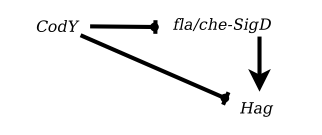
\includegraphics[scale=0.5]{wilkinson_reg_network.png}
\caption{Regulatory relationships. $Hag$ is the gene for $flagellin$, while $SigD$ encodes $\sigma^D$.}
\end{center}
\label{fig:}
\end{figure}


\begin{align*}
\end{align*}
\begin{align*}
\end{align*}
\begin{align*}
\end{align*}
\begin{align*}
\end{align*}

%\texttt{code snippet}
%
%\begin{algorithm}[h]
%\caption{ }
%Do things\\
%Loop:\\
%\Indp
% Do this again and again\\
%\end{algorithm}

%\begin{figure}[h!]
%\begin{center}
%\includegraphics[height=4in,width=6in]{filename.pdf}
%\caption{}
%\end{center}
%\label{fig:}
%\end{figure}

%$\left[
%\begin{tabular}{ >{$}c<{$} >{$}c<{$}}
% 1 & -\phi_1\\
% -\phi_1 & 1
%\end{tabular} 
%\right]$

%==== Bib files and style =======
\bibliographystyle{splncs}
\bibliography{prelim_biblio}
\end{document}
